
%%%%% To reason about%
In this chapter, we develop a new adaptivity analysis framework for
adaptive data analysis as in Figure~\ref{fig:structure}.
% There are mainly three parts, each targeting on a challenge above.
It is composed of three parts as well, with each part targeting on a challenge introduced in Chapter~\ref{sec:adapt-intro}.
The fundamental part is the {\tt Query While} language designed for formalizing the 
adaptive data analysis. Building on this, 
we formally define the intuitive \emph{adaptivity} 
and design a static program analysis algorithm for approximating the upper bound of the 
adaptivity as the two major parts of this framework.
This new framework improves the expressiveness, accuracy and the efficiency.
\begin{figure}
   \centering   
   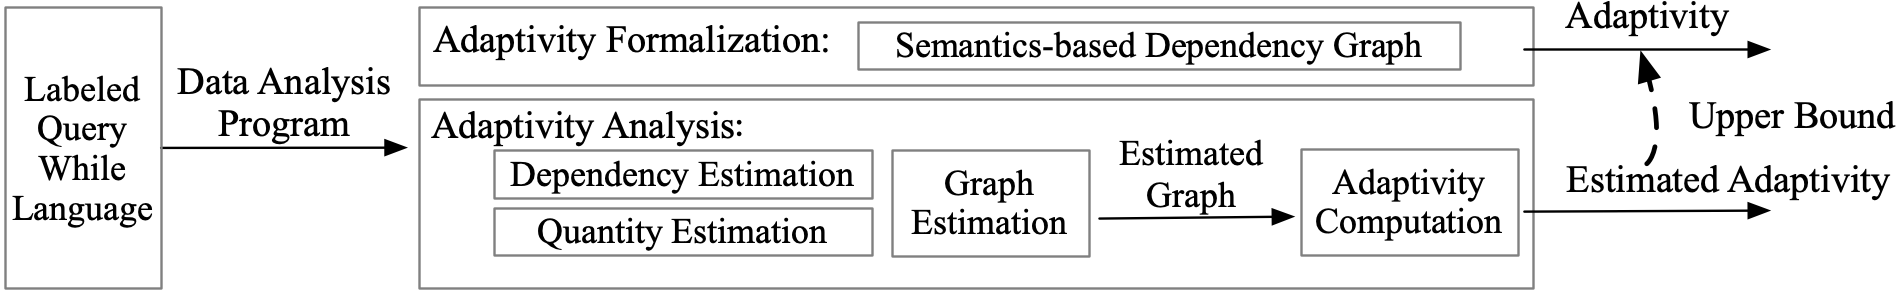
\includegraphics[width=1.0\textwidth]{figures/architecture}
  \caption{Architecture of The Adaptivity Analysis Framework}
   \label{fig:structure}
   \vspace{-1.0cm}
\end{figure}